\documentclass[11pt]{article}

% Packages

\usepackage{amsmath}
\usepackage{amssymb}
\usepackage{graphicx}

% Style

\newcommand{\Keywords}[1]{\vspace{12pt}\par\noindent
{\small{\bf Keywords\/}: #1}}
\renewcommand{\thesection}{\Roman{section}} 
\renewcommand{\thesubsection}{\thesection.\Alph{subsection}}
\renewcommand{\thesubsubsection}{\thesubsection.\arabic{subsection}}
\renewcommand{\thetable}{\Roman{table}}

% Helpers

\newcommand{\E}[1]{\times10^{#1}}
\newcommand{\A}[0]{\mathbb{A}}
\newcommand{\F}[0]{\mathbb{F}}
\newcommand{\M}[0]{\mathbb{M}}
\newcommand{\SRC}[0]{\mathbb{S}}
\newcommand{\braket}[2]{\left<#1\middle|#2\right>}
\newcommand{\brabiket}[3]{\left<{#1\left|#2\right|#3}\right>}
\newcommand{\iso}[2]{$^{#2}\mathrm{#1}$}
\newcommand{\tild}[0]{\sim\!\!}
\newcommand{\units}[1]{\left[\mathrm{#1}\right]}

\begin{document}

\title{Analysis of local void coefficients of reactivity in the reduced moderation BWR}
\author{Jeffrey E. Seifried \and Ehud Greenspan\footnote{Email: gehud@nuc.berkeley.edu}\\
\em University of California Berkeley\\
\em Department of Nuclear Engineering\\
\em 4155 Etcheverry Hall, MC 1730\\
\em Berkeley, CA 94720, USA
}
\date{}
\maketitle

\begin{abstract}
    An expression is derived for attributing the reactivity response due to perturbations to spectral, spatial, and isotopic effects.
    It is shown to be consistent at a global level with similar expressions derived in previous work, but can provide more detailed information on the physics phenomena contributing to the reactivity response of the perturbation.
    Using this expression, the reactivity effect of local coolant density perturbations -- local VCR -- are studied for two reduced-moderation BWR core designs: the RBWR-Th and RBWR-AC as well as for a standard ABWR.
    The RBWR core designs feature large axial variation in their neutron spectra.

    The axial distribution of local VCR along the RBWR-Th seed and along the ABWR core were found to have the same general shape: negative throughout but most negative near the bottom and asymptotically approaching zero towards the top.
    However, the RBWR-Th VCR is roughly 4 times more negative.
    The RBWR-AC local VCR axial distribution varies greatly -- it is very close to zero in the seed regions and has a significant positive component in the central blanket.

    Three effects were identified as contributing to the VCR due to a local water density change in the lower part of the RBWR-Th seed -- local spectrum hardening that tends to increase the local reproduction factor ($\eta_r$) of each of the fuel isotopes; a redistribution of the local neutron absorption between the fuel isotopes resulting in a shift of absorptions from higher to lower isotopic reproduction factors and, hence, to a reactivity loss; and an axial flux tilt across the core from axial zones of higher $\eta_r$ to axial zones of lower $\eta_r$ which makes another negative contribution to the reactivity worth of the perturbation.

    \Keywords{coefficients of reactivity, attribution, feedback}
\end{abstract}

\pagebreak

\section{Introduction}
\label{sec:intro}

Coefficients of reactivity are typically quantified for global perturbations such as a uniform $50K$ increase of fuel temperature or a $10\%$ decrease in coolant flow-rate within a flow channel.
Such perturbations can be thought of as the simultaneous occurrence of a set of local perturbations which, for small enough perturbations, are independent of one another.

In certain core types, such as the Reduced moderation Boiling Water Reactor (RBWR) \cite{ganda2012sst,takeda2007blt} core, local perturbations invoke either negative or positive reactivity responses depending on the axial location.
Even when the global reactivity coefficient is slightly negative, there exists the possibility for instability in such cores.
The objective of this work is to attribute the cause of a local reactivity response to their underlying physical mechanisms.
Understanding of these mechanisms provides useful insight which can guide an effective search for optimal core designs.
This work provides tools to conduct such an analysis and demonstrates their utility with three core designs.

In Section \ref{sec:derive}, an expression is derived for attributing reactivity responses -- either global or local -- to the spatial, spectral, and isotopic dependence of neutron fission and capture reactions.
Section \ref{sec:equiv} demonstrates that, on a global basis, this expression is equivalent to those derived in previous work, but on a local (e.g., spatial, spectral, or, isotopic) basis, it is more informative.
Section \ref{sec:rbwrth} uses this new derivation and other tools to study local coolant void perturbations in the thorium-fueled RBWR (RBWR-Th) \cite{ganda2012sst} unit cell, which is described in Section \ref{sec:model}.
Section \ref{sec:other} performs similar analyses for the uranium-fueled RBWR (RBWR-AC) \cite{takeda2007blt} and conventional Advanced Boiling Water Reactor (ABWR) unit cells \cite{fennern2007asr}.
Finally, the accuracy of estimating the reactivity response to global perturbations from the reactivity response to local perturbations is addressed in Section \ref{sec:accuracy}.

\section{An Expression for Attributing Reactivity to System Components}
\label{sec:derive}

For infinite systems, the multiplication factor (k) is defined as:
\begin{equation}
    k\equiv \frac{\F}{\A}
\end{equation}
where $\F$ and $\A$ -- the fission neutron birth rate and neutron absorption rate, respectively -- are defined as:
\begin{equation}
    \begin{split}
    \F \equiv \int_V d\vec{r} \int_0^\infty dE \int_{4\pi} d\vec\Omega \; \nu(\vec r, E) \Sigma_f(\vec r, E) \psi(\vec r, E, \vec\Omega) \\
    \A \equiv \int_V d\vec{r} \int_0^\infty dE \int_{4\pi} d\vec\Omega \; \Sigma_a(\vec r, E) \psi(\vec r, E, \vec\Omega)
    \end{split}
\end{equation}
where $\nu$, $\Sigma_f$, $\Sigma_a$, and $\psi$ are the number of neutrons born per fission, macroscopic fission and absorption cross sections, and neutron flux and $\vec r$, $E$, and $\vec\Omega$ are the spatial, spectral, and directional neutron phase-space coordinates.
Reactivity ($\rho$) is defined as:
\begin{equation}
    \rho \equiv \frac{k-1}{k} = 1-\frac{\A}{\F}.
\end{equation}

A coefficient of reactivity ($\alpha$) measures the linear effect of a perturbation of a parameter ($p$) upon $\rho$.
It can be estimated directly with finite difference using nominal and perturbed multiplication factors:
\begin{equation}
    \alpha \equiv \frac{\partial\rho}{\partial p}
    \approx \frac{\Delta \rho}{\Delta p}
    = \frac{1}{\Delta p} \frac{\Delta k}{k k^\prime}
    \label{eqn:kdiff}
\end{equation}
where $x^\prime$ denotes a perturbed quantity $x$ and $\Delta x = x^\prime - x$.
This will be referred to as the k-difference approach.
Alternatively, $\alpha$ can be expanded in $\F$ and $\A$ with the product rule:
\begin{equation}
    \alpha = \frac{\partial\rho}{\partial\F} \frac{\partial\F}{\partial p} + \frac{\partial\rho}{\partial\A} \frac{\partial\A}{\partial p}.
\end{equation}
In this second approach, while derivatives of $\rho$ can be evaluated analytically:
\begin{equation}
    \frac{\partial\rho}{\partial\F} = +\frac{1}{k\F} \quad \mathrm{and} \quad \frac{\partial\rho}{\partial\A} = -\frac{1}{k\A}
    \label{eqn:rhoAnal}
\end{equation}
it is formally possible to quantify the derivatives of $\F$ and $\A$ using perturbation theory \cite{greenspan1976dpt}:
\begin{equation}
    \begin{split}
    \frac{\partial\F}{\partial p} = \braket{\frac{\partial(\nu\Sigma_f)}{\partial p}}{\psi} - \brabiket{\psi^\dagger}{\frac{\partial\M}{\partial p}}{\psi} \\
    \M\psi = \SRC \quad \mathrm{and} \quad \M^\dagger \psi^\dagger = \SRC^\dagger = \frac{\partial\F}{\partial\psi}
    \end{split}
    \label{eqn:pertF}
\end{equation}
and:
\begin{equation}
    \begin{split}
    \frac{\partial\A}{\partial p} = \braket{\frac{\partial(\Sigma_a)}{\partial p}}{\psi} - \brabiket{\psi^\dagger}{\frac{\partial\M}{\partial p}}{\psi} \\
    \M\psi = \SRC \quad \mathrm{and} \quad \M^\dagger \psi^\dagger = \SRC^\dagger = \frac{\partial\A}{\partial\psi}
    \end{split}
    \label{eqn:pertA}
\end{equation}
where $\psi^\dagger$, $\M$, and $\SRC$ are the adjoint flux, neutron transport operator, and neutron source term and the bra-ket notation is used for inner products.
For critical systems, the neutron source term is the fission source term divided by k.
The adjoint transport equations in Equations \ref{eqn:pertF} and \ref{eqn:pertA} must be solved using Generalized Perturbation Theory, for which shortcut estimators for the adjoint distribution like the Iterated Fission Probability \cite[864-869]{henry1964nk} offer no assistance.
Solution of these equations requires the two adjoint sources to first be estimated using ordinary transport and then multiple fixed-source adjoint transport calculations.
The task is difficult and computationally expensive to perform accurately and convenient tools do not currently exist.
Consequently a direct perturbation approach, not based upon adjoint theory, is chosen for the present analysis.

For such a direct approach, second-order accuracy can be achieved by evaluating the derivatives of $\rho$ in Equation \ref{eqn:rhoAnal} at the nominal and perturbed states and taking the average (i.e., the trapezoidal rule) and derivatives in $\F$ and $\A$ can be estimated using finite difference:
\begin{equation}
    \alpha \approx \frac{1}{2} \left(\frac{1}{k^\prime \F^\prime} + \frac{1}{k\F}\right)\frac{\Delta \F}{\Delta p} - \frac{1}{2} \left(\frac{1}{k^\prime \A^\prime} + \frac{1}{k\A}\right)\frac{\Delta \A}{\Delta p}
\end{equation}
$\Delta\F$ and $\Delta\A$ are the total scalar differences in neutron birth and absorption rates; they are distributed over a multi-dimensional phase-space of geometric space, neutron energy, neutron direction, isotope, and reaction type.
They can be calculated from continuous integrals or summations over discrete regions ($\xi$) of that phase-space.
Because the difference of a sum of elements can be written as the sum of differences of those elements, $\Delta\F$ and $\Delta\A$ can be expressed in a more illustrative form:
\begin{equation}
    \Delta \F = \sum_\xi w_\xi \left(\F_\xi^\prime - \F_\xi \right) \quad \mathrm{and} \quad \Delta \A = \sum_\xi w_\xi \left(\A_\xi^\prime - \A_\xi\right)
\end{equation}
where $w_\xi$ is the width of a discrete region of $\xi$.
Written this way, distributions of $\alpha$ over $\xi$ can be found.
Each region in phase-space can be said to have its own contribution ($\alpha_\xi$) to the overall coefficient of reactivity:
\begin{equation}
    \alpha = \sum_\xi w_\xi \alpha_\xi
\end{equation}
where:
\begin{equation}
    \alpha_\xi \approx \frac{1}{2 \Delta p} \left[\left(\frac{1}{k^\prime \F^\prime} + \frac{1}{k\F}\right)\Delta \F_\xi - \left(\frac{1}{k^\prime \A^\prime} + \frac{1}{k\A}\right)\Delta \A_\xi \right].
    \label{eqn:alpha2}
\end{equation}
Particular insight can be gained by examining the $\Delta \F_\xi$ and $\Delta \A_\xi$ terms of Equation \ref{eqn:alpha2} in isolation, in addition to the net of the two terms.

In later sections, $\alpha_\xi$ will be summed over all but a single dimension, providing its distribution over spatial ($\alpha_r$), spectral ($\alpha_E$), nuclear reaction ($\alpha_x$), and isotopic ($\alpha_i$) bins.
For example, the spatial distribution of $\alpha$ can be calculated as:
\begin{equation}
    \alpha_r = \sum_{E,x,i} \alpha_\xi  = \sum_{E,x,i} \alpha_{r,E,x,i}
\end{equation}
This $r/E/x/i$ subscript notation will also be used for other quantities which are distributed over $\xi$.

\section{Equivalency with Absorption and Fission Normalization Derivations}
\label{sec:equiv}

In past work, expressions for attributing coefficients of reactivity have been derived using so called absorption and fission normalizations \cite{ganda2010sst}.
This section shows that these two previous derivations for coefficients of reactivity ($\alpha_\A$ and $\alpha_\F$ respectively) are equivalent to the first-order portion of Equation \ref{eqn:alpha2} ($\alpha_1$) when each expression is summed over $\xi$.
Before this comparison can be made, Equation \ref{eqn:alpha2} is rearranged into a first-order term:
\begin{equation}
    \alpha_{\xi,1} = \frac{1}{\Delta p} \left[\frac{\Delta\F_\xi}{k^\prime\F} - \frac{\Delta\A_\xi}{k\A}\right]
    \label{eqn:alpha1}
\end{equation}
and a second-order term:
\begin{equation}
    \alpha_{\xi,2} = \frac{1}{2\Delta p} \left[\left(\frac{\Delta k}{k} - \frac{\Delta\F}{\F^\prime}\right)\frac{\Delta\F_\xi}{k^\prime \F} + \left(\frac{\Delta\F}{\F^\prime}\right)\frac{\Delta\A_\xi}{k\A}\right].
\end{equation}
The $\alpha_{\xi,2}$ expression is said to be second-order because its terms contain products of differences terms.

In order to derive $\alpha_\A$, perturbed and nominal neutron birth rate distributions are first normalized by the rate of neutrons absorbed in the system and then subtracted:
\begin{equation}
    \Delta k_{\xi,\A} \equiv \frac{\F_\xi^\prime}{\A^\prime} - \frac{\F_\xi}{\A} = k^\prime \frac{\F_\xi^\prime}{\F^\prime} - k \frac{\F_\xi}{\F}.
\end{equation}
Next, equal terms ($k \frac{\F_\xi^\prime}{\F} = k^\prime \frac{\F_\xi^\prime}{\F^\prime} \frac{\A^\prime}{\A}$) are added and subtracted:
\begin{equation}
    \begin{split}
        \Delta k_{\xi,\A}=\left(k \frac{\F_\xi^\prime}{\F} - k \frac{\F_\xi}{\F}\right) + \left(k^\prime \frac{\F_\xi^\prime}{\F^\prime}\frac{\A}{\A} - k^\prime \frac{\F_\xi^\prime}{\F^\prime}\frac{\A^\prime}{\A}\right) \\
        = k \frac{\Delta\F_\xi}{\F} - k^\prime \frac{\F_\xi^\prime}{\F^\prime}\frac{\Delta\A}{\A}.
    \end{split}
\end{equation}
Finally, upon invoking Equation \ref{eqn:kdiff}, the absorption-normalized expression for attribution is found:
\begin{equation}
    \alpha_{\xi,\A} = \frac{1}{\Delta p} \left[\frac{\Delta\F_\xi}{k^\prime \F} - \frac{\F_\xi^\prime}{\F^\prime} \frac{\Delta\A}{k\A}\right].
    \label{eqn:alphaA}
\end{equation}

In order to derive $\alpha_\F$, perturbed and nominal neutron absorption rate distributions are first normalized by the rate of neutrons born in the system and then subtracted:
\begin{equation}
    \Delta \rho_{\xi,\F} \equiv -\frac{\A_\xi^\prime}{\F^\prime} + \frac{\A_\xi}{\F} = -\frac{1}{k^\prime}\frac{\A_\xi^\prime}{\A^\prime} + \frac{1}{k}\frac{\A_\xi}{\A}.
\end{equation}
Next, equal terms ($\frac{1}{k} \frac{\A_\xi^\prime}{\A} = \frac{1}{k^\prime}\frac{\A_\xi^\prime}{\A^\prime}\frac{\F^\prime}{\F}$) are added and subtracted:
\begin{equation}
    \begin{split}
        \Delta \rho_{\xi,\F} = \left(\frac{1}{k^\prime}\frac{\A_\xi^\prime}{\A^\prime}\frac{\F^\prime}{\F} - \frac{1}{k^\prime}\frac{\A_\xi^\prime}{\A^\prime}\frac{\F}{\F}\right) - \left(\frac{1}{k}\frac{\A_\xi^\prime}{\A} - \frac{1}{k}\frac{\A_\xi}{\A}\right) \\
        = \frac{1}{k^\prime}\frac{\A_\xi^\prime}{\A^\prime}\frac{\Delta\F}{\F} - \frac{1}{k}\frac{\Delta\A_\xi}{\A}.
    \end{split}
\end{equation}
Finally, upon invoking Equation \ref{eqn:kdiff}, the fission-normalized expression for attribution is found:
\begin{equation}
    \alpha_{\xi,\F} = \frac{1}{\Delta p}\left[\frac{\A_\xi^\prime}{\A^\prime}\frac{\Delta\F}{k^\prime \F} - \frac{\Delta\A_\xi}{k\A}\right].
    \label{eqn:alphaF}
\end{equation}

While there are differences between the expressions for $\alpha_{\xi,\A}$, $\alpha_{\xi,\F}$, and $\alpha_{\xi,1}$ (Equations \ref{eqn:alpha1}, \ref{eqn:alphaA}, and \ref{eqn:alphaF}, respectively), when each is summed over $\xi$, the resulting expressions for $\alpha_\A$, $\alpha_\F$, and $\alpha_1$ are identical to each other and equal to the result given by k-difference approach (Equation \ref{eqn:kdiff}).
Although the three approaches are globally equivalent, $\alpha_{\xi,\A}$ cannot resolve contributions from $\Delta\A$ across $\xi$ because it only accounts for the total absorption rate and not its distribution.
Likewise, $\alpha_{\xi,\F}$ cannot resolve contributions from $\Delta\F$ across $\xi$ because it accounts for the total fission rate and not its distribution.
$\alpha_{\xi,1}$ and $\alpha_{\xi,2}$, on the other hand, account for the local contribution of both absorption and fission changes so that correct sign and magnitude can be attributed to each component.

\section{Description of the RBWR-Th Unit Cell}
\label{sec:model}

The RBWR-Th \cite{ganda2012sst} is a thorium fueled self-sustaining RBWR -- a design variant of the depleted uranium fueled self-sustaining RBWR-AC designed by HITACHI to fit within the ABWR pressure vessel \cite{takeda2007blt}.
The RBWR-Th departs from the RBWR-AC in several ways: thorium is used as the fertile fuel instead of depleted uranium, the internal axial blanket is eliminated elongating the fissile region, and absorbers in the upper and lower reflectors are removed.

As the present study focuses on the axial variation of the void coefficient of reactivity, the RBWR-Th core is modeled with a single pin unit cell consisting of a $1.005cm$ OD fuel pin segmented into a $50cm$ long lower blanket, a $111cm$ long central seed, and a $70cm$ long upper blanket and arranged in a hexagonal lattice of pitch $1.135cm$.
The mixed oxide fuel is assumed to be at $90\%$ of its nominal density ($0.061[a/b-cm]$) and is clad with $0.06cm$ thick metallic zirconium ($0.043[a/b-cm]$).
Fuel and clad are assumed to be at $900K$.
Lower and upper reflectors are modeled as pure water of a density corresponding to, respectively, the coolant inlet to and exit from the core.
Side and top views of the unit cell are shown in Fig. \ref{fig:xport}.

Before each cycle, blankets are charged with natural thoria and the seed is charged with the processed transthoria discharge harvested from the seed and blankets of the previous cycle.
During this fuel processing, all actinides are recycled and fission products are discarded.
All analysis is performed at fuel cycle equilibrium, when the charge of each successive cycle is the same.
Table \ref{tab:iso} shows the isotopic composition of the seed fuel region which is used.
MCNP6.1 is used for all neutron transport calculations \cite{lanl2013mcnp6}.

Because accurate determination of the RBWR-Th core performance requires tight coupling between neutronics and thermal/hydraulics, a one-dimensional heat balance and drift-flux model is coupled with neutron transport calculations to ensure that the axial distributions of two-phase coolant density and fission power are self-consistent across $57$ axial regions \cite{seifried2013aec}.
Each fuel pin provides $20kW$ of thermal power to boil the light water coolant -- which enters the core at $7.25MPa$ and $278.5 ^\circ C$ -- to an exit quality of $35\%$ corresponding to a void fraction of $\tild 80\%$.
For this model, a modified version of the Liao, Parlos, Griffith void fraction correlation is used \cite{shirvan2013bev}.

Fig. \ref{fig:rho} and Fig. \ref{fig:lhr} show the axial distribution of the water density and linear heat rate.
The region below $50cm$ is the lower blanket, above $161cm$ is the upper blanket, and in between is the seed.
The large differences in water density cause the neutron spectra to vary greatly along the core.
Fig. \ref{fig:flx} shows a typical flux spectrum for the RBWR-Th and compares it with that of the RBWR-AC, the ABWR, and a typical Sodium Fast Reactor (SFR).
The RBWR cores have intermediate flux spectra which are not as soft as the ABWR and not as hard as the SFR.

\section{Local Void Coefficients of Reactivity in the RBWR-Th}
\label{sec:rbwrth}

The local void coefficient of reactivity, or local VCR, is the linear reactivity response to a localized perturbation in the coolant density.
Such perturbations are estimated with a $10\%$ reduction in coolant density for a single axial region.
The coolant and fuel are segmented into $10$, $30$, and $15$ axial regions for the lower blanket, seed, and upper blanket regions, respectively.
VCRs are reported in pcm per $1\%$ increase in coolant void (or $1\%$ decrease in coolant density).

First, local VCRs are calculated using KPERT, a new tool in MCNP6.1 which is designed for efficient estimation of the reactivity response to perturbations \cite{kiedrowski2011awt}.
Although its accuracy can be limited for drastic perturbations, KPERT is very effective for quickly indicating trends and guiding attention to important spatial locations or isotopes.
In the same runtime required for a k-difference approach to calculate the reactivity effect of one perturbation, KPERT can simulate more than $50$.
MCNP also has an older perturbation tool PERT which does not perform as well as KPERT.
Fig. \ref{fig:verify} compares the k-difference estimates of the KPERT and PERT to direct k-difference calculations.
While KPERT results lie just outside of the error bars, PERT predictions differ by $\tild 1/3$ or more.
This is likely due to the large flux redistribution which occurs during the perturbation at position $b$, which KPERT can account for, but PERT cannot.
These conclusions were also found in other calculations.

More accurate and thorough direct analysis is then performed for coolant density perturbations at selected locations found of interest using the expressions for reactivity attribution derived in Sections \ref{sec:derive} and \ref{sec:equiv}.
Additional insight is gained by examining local reproduction factors (i.e., $\eta_r \equiv \frac{\F_r}{\A_r}$) and utilization factors (i.e., $f_r \equiv \frac{\A_r}{\A}$).
With this set of analyses, the cause for negative and positive local VCRs can be attributed to underlying physics in the RBWR-Th core.

Fig. \ref{fig:kpert} displays the local VCRs for the RBWR-Th core at Beginning Of Equilibrium Cycle calculated with KPERT.
It can be seen that local VCRs vary strongly along the core; they are negative along the seed region -- particularly so in its lower, softer spectrum part, while slightly positive in the blankets -- particularly adjacent to the seed.
Two local perturbations were selected for deeper analysis aimed at understanding the underlying physics: (a) the most positive local VCR within the lower blanket adjacent to the seed and ($b$) the most negative local VCR within the seed towards the inlet.
Perturbation $b$ is discussed first.

\subsection{The Most Negative Local VCR Within the RBWR-Th}
\subsubsection{Comparison of Different Formulations for VCR for Spatial Components}

Using expressions for $\alpha_\A$ and $\alpha_\F$ (Equations \ref{eqn:alphaA} and 21), the contribution of different axial zones to perturbation $b$'s VCR -- the VCR due to coolant density change in location $b$, were quantified and displayed in, respectively, Fig. \ref{fig:alphaAR} and Fig. \ref{fig:alphaFR}.
It is found that both $\F$ and $\A$ are depressed in the vicinity of the perturbation and $\F$ and $\A$ both shift away from the perturbation towards the outlet.
The first response will be shown due to localized spectral hardening resulting in a reduced fission probability and the second due to flux tilt caused by normalization by $\A$ and $\F$ rates.

Fig. \ref{fig:alpha1R} and Fig. \ref{fig:alpha2R} display the first- and second-order predictions for axial contributions to the overall local VCR from perturbation $b$, obtained using, respectively, Equations \ref{eqn:alpha1} and \ref{eqn:alpha2}.
As in case of $\alpha_\A$ and $\alpha_\F$, there are local spectral hardening effects and global flux tilt effects.
Spectral hardening has a net negative reactivity effect due to a localized reduction in the reproduction factor.
This is illustrated in Fig. \ref{fig:deltaEtaR} which plots the change in the location-dependent $\eta_r$ due to perturbation $b$.
The flux tilt also results in a net negative effect due to a spatial shift in the local utilization factor shown in Fig. \ref{fig:deltaEffR} as shown in Fig. \ref{fig:etaR} $\eta_r$ is highest near the core inlet where the flux spectrum is softest and decreases with elevation as the spectrum hardens with reduction in the coolant density.
As a result, $\sum_r{\eta_r\Delta f_r}$ is negative.
Although the two responses cannot be isolated, it is estimated that $60\%$ of the total reactivity effect is from spectrum hardening ($\sum_r{\Delta\eta_r f_r}$) and $40\%$ is from the flux tilt ($\sum_r{\eta_r \Delta f_r}$).

The k-difference approach estimates the overall local VCR for perturbation $b$ to be $-6.8 \pm 0.5 [pcm/\%-void]$.
In Table \ref{tab:deltaAlpha} the deviations between this estimate those of $\alpha_\A$, $\alpha_\F$, $\alpha_1$, and $\alpha_2$ are tabulated.
The associated p-values (i.e., the probability of observing the deviation given that there is no true deviation) demonstrate that these deviations are completely insignificant (i.e., $p>>5\%$), so all five approaches predict the same overall local VCR.
This conclusion was expected from inspection of the algebraic expressions.

The expressions do differ, however, in predicting the components (spatial, spectral, isotopic) of the reactivity.
For example, the contribution of the flux tilt in the upper region of the seed is positive as estimated with $\alpha_\A$ (Fig. \ref{fig:alphaAR}), but negative as estimated with $\alpha_\F$ (Fig. \ref{fig:alphaFR}).
$\alpha_1$ and $\alpha_2$, however, show that the region has an increase in both absorption and fission, but contributes practically no net reactivity worth.
This comparison brings to light a shortcoming of the $\alpha_\A$ and $\alpha_\F$ expressions, for examining components of the reactivity.

Although $\alpha_2$ is believed to be more accurate in estimating components of reactivity than $\alpha_1$ by virtue of its second-order terms, there currently is no benchmark to compare against.
Nonetheless, a comparison is made between the two expressions to quantify the magnitude of the second-order terms; the result is shown in Fig. \ref{fig:deltaAlphaR}.
Relative to $\alpha_1$,  $\alpha_2$ is estimating: 1) less positive and less negative contributions from changes in fission and absorption, respectively; 2) an enhanced, more negative contribution from the seed region; and 3) a reduced, less negative contribution from the blankets.
All following $\alpha_\xi$ values and distributions will be derived from the $\alpha_2$ expression.

\subsubsection{Isotopic Contributions}

The spectral hardening effect is further explored by examining $\alpha_\xi$ in the proximity of perturbation $b$ (the five axial regions bordering it), but binned over isotope ($i$) instead of axial region.
Fig. \ref{fig:alpha2I} displays these results for the isotopes which provide the largest reactivity worth.
It can be seen that fissile isotopes -- predominately \iso{U}{233}, \iso{U}{235} and \iso{Pu}{239} -- contribute a net negative reactivity, while non-fissile isotopes -- predominately \iso{Th}{232}, \iso{U}{234}, and \iso{U}{236} -- contribute a net positive reactivity.
Both classes of isotopes exhibit reductions in $\F$ and $\A$, but the reduction in $\F$ of \iso{U}{233} is the dominant.
Coolant and clad materials do not play a significant role in the reactivity response to perturbation $b$, contributing less than $5\%$ of the total worth.

Fig. \ref{fig:deltaEtaI} shows that spectral hardening increases isotopic $\eta_i$ values near perturbation $b$.
In order to understand the change in $\eta_i$ of the mixture of fuel isotopes, the perturbation effect on isotopic $f_i$ must also be considered.
Fig. \ref{fig:etaI} plots the $\eta_i$ value for each isotope and Fig. \ref{fig:deltaEffI} shows the changes in isotopic $f_i$ values which result from perturbation $b$, plotted over the same abscissa.
Even though the perturbation increases the $\eta_i$ values for every isotope, the net reactivity effect ($\sum_i{\Delta\eta_i f_i} + \sum_i{\eta_i \Delta f_i}$) is reduced by $185 \pm 31 [pcm]$.
This is because the perturbation shifts absorptions from higher $\eta_i$ (such as \iso{U}{233}) to lower $\eta_i$ such as \iso{U}{234}).
If the effect of \iso{U}{233} is excluded, the trend reverses and the change in the overall $\eta_i$ becomes slightly positive. 

The underlying mechanisms which cause negative reactivity due to spectral hardening and flux tilt are identical: $f_i$ values shift from a phase-space of higher to lower $\eta_i$ values.
For the flux tilt response, that phase-space is axial position; for the spectral hardening response, the phase-space is isotopes in proximity to the perturbation.
Further insight can be obtained by studying the spectral characteristics of this latter response.

\subsubsection{Spectral Components}

Fig. \ref{fig:deltaFlx} shows the spectral hardening due to perturbation $b$, considering only those five axial regions which border perturbation $b$.
The flux shifts to the energy range between $10 keV$ and $1 MeV$ from, epithermal energies -- due to a reduced moderating power, and from above $1 MeV$ due to a reduced local fission rate and due to enhanced inelastic scattering probability by the fuel.
Fig. \ref{fig:alphaETh} and Fig. \ref{fig:alphaEU} show the impact these spectral changes have upon $\eta_E$ values for \iso{Th}{232} and \iso{U}{233} in proximity of perturbation $b$, as a function of the neutron energy. \iso{Th}{232} contributes a large increase in reactivity due to, primarily, a reduction in resonance absorption.
The slight reduction in the \iso{Th}{232} fast fission probability has only a very small negative effect on the reactivity coefficient.
The overall decrease in the neutron absorption probability due to local voiding is responsible for the net positive contribution to the reactivity worth of the other non-fissile isotopes as well.

Fig. \ref{fig:alphaEU} shows the energy-dependent contributions of \iso{U}{233} to the reactivity coefficient via the spectral effects on the absorption and fission probabilities.
It is observed that the spectrum hardening results in a significant increase in both the neutron absorption and neutron fission probabilities in, primarily, the epithermal energy range but the latter effect is dominant so the net reactivity worth is negative.
This trend also applies to each of the other fissile isotopes.

From the perspective of $f_E$ and $\eta_E$ values -- Fig. \ref{fig:deltaFlx} shows that the perturbation shifts spectral $f_E$ from, primarily, epithermal but also thermal and MeV energies to sub-MeV energies.
From examination of the energy dependence of the absorption cross section of the two most absorbing fuel isotopes in the RBWR-Th core displayed in Fig. \ref{fig:xs} it is expected that this redistribution shifts the local absorptions from primarily \iso{U}{233} to primarily \iso{Th}{232} which has a significantly lower $\eta_E$ value, thus reducing the local reactivity effect.

In summary, perturbation $b$ causes a spatial redistribution of power, which shifts flux away from axial regions with higher $\eta_r$ values and towards those with lower $\eta_r$ values.
Additionally, the perturbation causes localized spectral hardening which shifts absorption from isotopes with higher $\eta_i$ values to those with lower $\eta_i$ values, reducing the axial $\eta_r$ value in the vicinity of the perturbation.
While this spectral hardening also tends to increase localized $\eta_r$ values somewhat, the absorption redistribution is a larger effect.
Both the flux tilt and spectral hardening responses bring a negative reactivity worth, for an overall strong negative local VCR.

\subsection{The Most Positive Local VCR Within the RBWR-Th}

Perturbation $a$ is a reduction in the coolant density in axial zone a of the lower blanket that is close to the seed.
This voiding causes both a streaming response -- which has a very small reactivity effect -- and a flux tilt response -- which has a net positive reactivity worth.
The two responses can be resolved in Fig. \ref{fig:deltaEffRb}, which shows the change in axial $f_r$ due to perturbation $a$.

The streaming response is characterized by a reduced albedo of the lower blanket to neutrons that are generated in the seed and happen to leak into the lower blanket; the voided coolant increases the number of seed-born neutrons that stream beyond perturbation $a$, causing $f_r$ to shift downwards.
As can be seen in Fig. \ref{fig:etaR} the $\eta_r$ within this region of the blanket is negligibly small compared to the rest of the system (it is a fertile blanket, after all), so the spatial shift in $f_r$ brings no significant reactivity change.

The flux tilt response is similar to that from perturbation $b$, except that the seed power shifts downwards instead of upwards (Fig. \ref{fig:deltaEffR}).
The downwards flux tilt shifts local $f_r$ values from axial regions of lower to higher $\eta_r$ values (Fig. \ref{fig:etaR}).
The result is an increase in the effective $\eta$ (i.e., $\frac{\sum_r{\eta_r f_r}}{\sum_r{f_r}}$) for the system and, hence, a reactivity gain.
The localized spectral hardening response which was seen in the RBWR-Th system can't quite be resolved within the statistical uncertainty.
However, it is estimated that its contribution is negative and one-fifth the magnitude of the power-tilt response.

\section{Local Void Coefficients of Reactivity in the ABWR and RBWR-AC}
\label{sec:other}

The RBWR-Th inherits many of its core design features from the ABWR \cite{fennern2007asr} and RBWR-AC \cite{takeda2007blt}.
Following is a comparative local VCR analysis of the three systems; it can provide useful information on the uniqueness of the RBWR-Th core design.

Fig. \ref{fig:kpertAbwr} shows the axial distribution of ABWR local VCRs, as estimated with KPERT.
Comparing with Fig. \ref{fig:kpert} it is seen that the ABWR and RBWR-Th local VCRs have the same general shape: (1) both are negative throughout the active length of the seed fuel; (2) local VCRs are most negative in the lower quadrant of the active length; and (3) local VCRs asymptotically approach zero towards the outlet.
However, the RBWR-Th VCR gets to be $\tild 4$ times more negative and this may be of practical concern as it may cause instabilities and make it difficult to achieve adequate cold shutdown margin.
A recent study found \cite{gorman2014tfr} that by replacing $1/4$ to $1/3$ of the thorium of the makeup fuel by depleted uranium it is possible to make the VCR comparable in magnitude to that of the ABWR.

Fig. \ref{fig:kpertAc} plots the local VCR traverse for the RBWR-AC \cite{takeda2007blt}, as estimated with KPERT.
This VCR distribution differs greatly from that of the RBWR-Th (Fig. \ref{fig:kpert}) except for one feature: a sharp local minimum close to the bottom of each seed region.
But in the RBWR-AC the VCR does not have significant negative components; in fact, its average is close to a value of zero.
The RBWR-AC has large positive VCR values within the internal and upper blankets adjacent to the seeds but negative values at the bottom blanket.
The large VCR values in the RBWR-AC blankets are due to the use of depleted uranium fuel; \iso{U}{238} has a larger fast fission cross section than \iso{Th}{232} and its threshold energy is lower.
The most positive local perturbation $b$ at the bottom of the inner blanket is chosen for limited attribution analysis.

Fig. \ref{fig:alphaAc} shows the contribution to local VCR from all axial fuel regions.
The axial variations are significantly more complicated than those in the RBWR-Th -- (Fig. \ref{fig:alpha2R}).
Fig. \ref{fig:spectralAc} shows the axial spectral hardening response; it has noticeable components from the RBWR-AC lower seed and internal blanket axial zones in the proximity of the perturbed zone.
Fig. \ref{fig:tiltAc} shows that the axial extent of the flux tilt response is much wider -- from the bottom blanket to the upper seed.
Reduction in the coolant absorption probability contributes around one fifth of the reactivity effect.

Due to the complicated reactivity responses, it is difficult to isolate the spectral hardening and flux tilt responses from one another.
However, by summing over values in the two figures, it is estimated that localized spectral hardening is responsible for one-fifth of the local VCR and flux tilting contributes the other fourth-fifths.

A more thorough analysis of the local VCRs in the RBWR-AC core using the analysis methodology developed in this study, along with prolonged runtimes to reduce counting uncertainty, could help identifying RBWR-AC core designs that feature negative void coefficient of reactivity.

\section{Accuracy of the Linear Combination of Local Perturbations}
\label{sec:accuracy}

A primary assertion made in this work is that there is value in studying the reactivity response from local perturbations because their combined effect is a reasonable estimate of the global reactivity effect of the perturbations.
If this assertion is correct it is possible to construct a large number of global perturbations by linearly combining the effects of different combinations of local perturbations.
This section provides a simple sanity check by comparing the direct reactivity effect from a coolant flow-rate reduction with that estimated from linearly combining local void perturbations.

The direct estimate begins by iterating between neutron transport and thermal/hydraulic solutions until a tight convergence is obtained between the axial water density and axial power shape \cite{seifried2013aec}.
This is performed at the nominal flow conditions and at a $10\%$ reduced coolant flow-rate.
Multiplication factors for the nominal and perturbed state are extracted and plugged into Equation \ref{eqn:kdiff} for the coolant flow-rate coefficient of reactivity (FRCR).
The combined FRCR is calculated by taking the inner product of a system's local VCR traverse with the change in the void fraction traverse which results from the coolant flow-rate reduction and dividing by $10\%$.
The latter will be referred to as the inner product approach.
KPERT was used for estimating local VCR traverses.
Its accuracy can be inferred from the results provided in Fig. \ref{fig:verify}.

For the RBWR-Th the FRCR was calculated to be $-67.2 \pm 0.1 [pcm/\%]$ using the k-difference approach and $2.3 \pm 0.8\%$ (2.9 standard deviations) lower using the inner product approach.
For the RBWR-AC, the k-difference FRCR is $-2.7 \pm 0.1 [pcm/\%]$ while the inner product approach gave an estimate of $-1.8 \pm 0.4 [pcm/\%]$ that is $35 \pm 20\%$ too low.
This is probably due to strong non-linear effects in the strongly axially heterogeneous RBWR-AC core.

For typical core designs that feature a single seed zone agreement between the inner product and the k-difference approaches is quite good.
Because the inner product approach can provide estimates for a number of perturbations with the same runtime required for one k calculation, it is an efficient approach for scoping studies. 

\section{Conclusions}
\label{sec:conclusion}

The expressions derived for estimating the reactivity effect of perturbations provide informative estimates of the total reactivity effect and of its components.
The methodology developed to quantify the spectral and flux tilt contributions to the reactivity effects of localized perturbations provide useful insight on the physics phenomena at play.
Additional useful insight is provided by quantifying the contribution to the reactivity effect of individual fuel isotopes and of the spectral and spatial components of this contribution.
Expressions derived in past work by absorption and fission normalization yield the same total reactivities, but can provide misleading information on the contribution of different phase-space variables to the global reactivity.

The axial distribution of local VCR along the RBWR-Th seed and along the ABWR core have the same general shape: negative throughout but most negative in the lower quadrant of the active length; the local VCRs asymptotically approach zero towards the outlet.
However, the RBWR-Th VCR gets to be $\tild 4$ times more negative and this may be of practical concern as it may cause instabilities and make it difficult to achieve adequate cold shutdown margin.
The RBWR-AC local VCR axial distribution differs greatly from that of the other two core types -- it is very close to zero in the seed regions and has a significant positive component in the central blanket.

Three types of spectral effects were identified contributing to the VCR due to a local water density change in the lower part of the RBWR-Th seed -- local spectrum hardening that tends to increase the local reproduction factor ($\eta$) of each of the fuel isotopes; a redistribution of the local neutron absorption between the fuel isotopes resulting in a shift of absorptions from higher $\eta_i$ to lower $\eta_i$ isotopes and, hence, to a reactivity loss; and axial flux tilt across the core from axial zones of higher $\eta_r$ to axial zones of lower $\eta_r$ which makes another negative contribution to the reactivity worth of the perturbation.
The underlying mechanisms which cause negative reactivity due to the latter two effects are identical: $f_\xi$ values shift from a phase-space $\xi$ of higher $\eta_\xi$ to a phase-space of lower $\eta_\xi$ values.

The KPERT tool was found to be very effective at providing accurate estimates for the reactivity response from local perturbations.
A limited check showed that linear superposition of the reactivity effect of local perturbations provides a good estimation of the global perturbation reactivity effect for the RBWR-Th.
This is also expected to be the case for the ABWR core but not for the RBWR-AC core which is more sensitive to axial power tilts due to its unique heterogeneity.
A more thorough study to understand the shortcomings of the approach is warranted.

\section{Acknowledgements}

This research was performed using funding received from the U.S. Department of Energy Office of Nuclear Energy's Nuclear Energy University Programs.
This material is based upon work supported by the U.S. Department of Energy National Nuclear Security Administration under Award Number DE-NA0000979.

\appendix
\bibliographystyle{ans}
\bibliography{NSE14-104}

\clearpage
\begin{figure}[p]
  \centering
  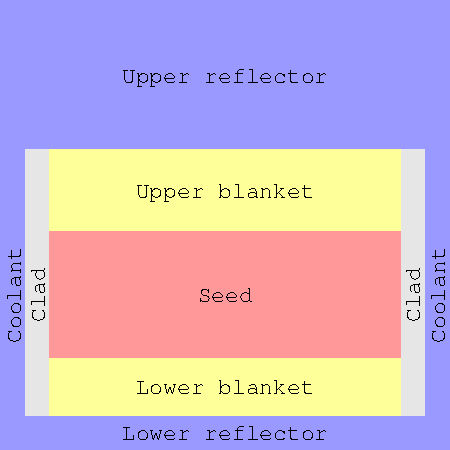
\includegraphics[width=0.45\textwidth, trim=0 0 0 0, clip]{./img/Th-xportSide.pdf}
  \hspace{0.1in}
  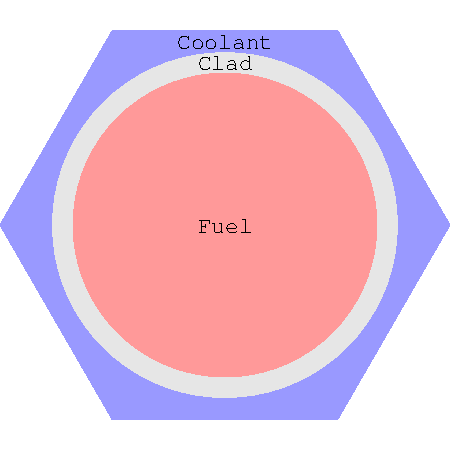
\includegraphics[width=0.45\textwidth, trim=0 0 0 0, clip]{./img/Th-xportTop.pdf}
  \caption{The RBWR-Th single-pin unit cell shown (left) from the side and (right) from above. Figures are not to scale.}
  \label{fig:xport}
\end{figure}

\clearpage
\begin{table}[ht]
    \centering
    \caption{Isotopic composition of the seed fuel region for the RBWR-Th single-pin unit cell.}
    \label{tab:iso}
    \begin{tabular}{| c | c | c |} \hline
    \textbf{Isotope} & \textbf{Number Density} \\
                     & \textbf{$[a/b/cm]$}     \\ \hline
    \iso{O}{16}      & $4.1259\E{-2}$          \\ \hline
    \iso{Th}{228}    & $7.5461\E{-7}$          \\ \hline
    \iso{Th}{229}    & $3.4110\E{-7}$          \\ \hline
    \iso{Th}{230}    & $7.9693\E{-7}$          \\ \hline
    \iso{Th}{232}    & $1.7153\E{-2}$          \\ \hline
    \iso{Pa}{231}    & $1.2033\E{-5}$          \\ \hline
    \iso{U}{232}     & $2.9986\E{-5}$          \\ \hline
    \iso{U}{233}     & $1.4777\E{-3}$          \\ \hline
    \iso{U}{234}     & $1.0605\E{-3}$          \\ \hline
    \iso{U}{235}     & $2.5392\E{-4}$          \\ \hline
    \iso{U}{236}     & $3.1760\E{-4}$          \\ \hline
    \iso{U}{238}     & $4.1905\E{-7}$          \\ \hline
    \iso{Np}{236}    & $4.7333\E{-9}$          \\ \hline
    \iso{Np}{237}    & $7.3786\E{-5}$          \\ \hline
    \iso{Pu}{238}    & $1.6406\E{-4}$          \\ \hline
    \iso{Pu}{239}    & $4.2105\E{-5}$          \\ \hline
    \iso{Pu}{240}    & $1.5521\E{-5}$          \\ \hline
    \iso{Pu}{241}    & $9.1368\E{-6}$          \\ \hline
    \iso{Pu}{242}    & $4.4926\E{-6}$          \\ \hline
    \iso{Pu}{244}    & $3.2513\E{-9}$          \\ \hline
    \iso{Am}{241}    & $4.2129\E{-6}$          \\ \hline
    \iso{Am}{242}    & $2.9638\E{-7}$          \\ \hline
    \iso{Am}{243}    & $1.8736\E{-6}$          \\ \hline
    \iso{Cm}{242}    & $3.0946\E{-9}$          \\ \hline
    \iso{Cm}{243}    & $1.5450\E{-7}$          \\ \hline
    \iso{Cm}{244}    & $2.6789\E{-6}$          \\ \hline
    \iso{Cm}{245}    & $1.8284\E{-6}$          \\ \hline
    \iso{Cm}{246}    & $1.5318\E{-6}$          \\ \hline
    \iso{Cm}{247}    & $2.5120\E{-7}$          \\ \hline
    \iso{Cm}{248}    & $2.5165\E{-7}$          \\ \hline
    \iso{Cf}{249}    & $6.0420\E{-8}$          \\ \hline
    \iso{Cf}{250}    & $9.3489\E{-9}$          \\ \hline
    \iso{Cf}{251}    & $1.0228\E{-8}$          \\ \hline
    \iso{Cf}{252}    & $8.4902\E{-10}$         \\ \hline
    \end{tabular}
\end{table}

\clearpage
\begin{figure}[p]
  \centering
  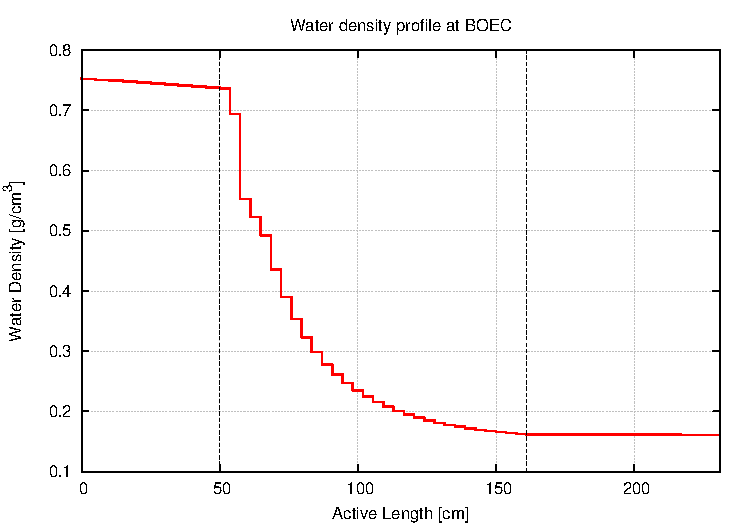
\includegraphics[width=\textwidth, trim=0 0 0 0.275in, clip]{./img/Th-waterDensity.pdf}
  \caption{Axial distribution of the RBWR-Th water density.}
  \label{fig:rho}
\end{figure}

\clearpage
\begin{figure}[p]
  \centering
  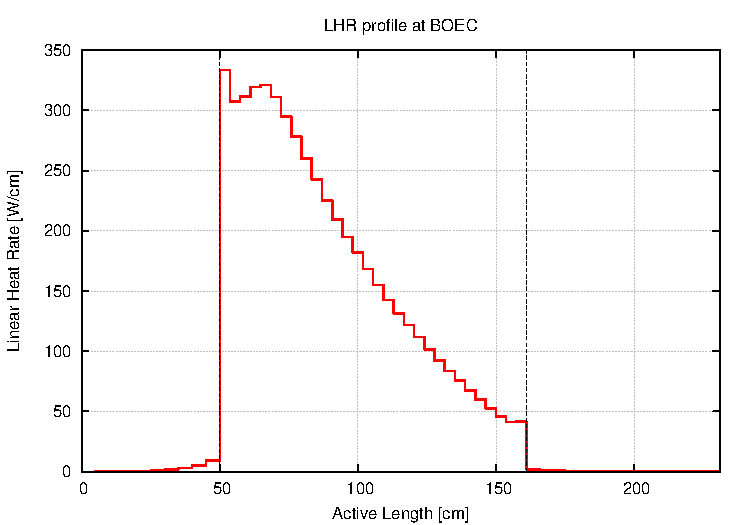
\includegraphics[width=\textwidth, trim=0 0 0 0.275in, clip]{./img/Th-lhr.pdf}
  \caption{Axial distribution of the RBWR-Th linear heat rate.}
  \label{fig:lhr}
\end{figure}

\clearpage
\begin{figure}[p]
  \centering
  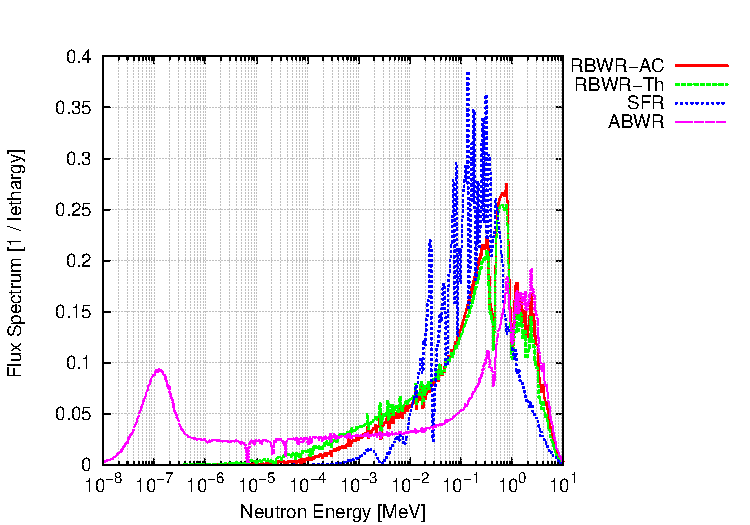
\includegraphics[width=\textwidth, trim=0 0 0 0.275in, clip]{./img/fluxSpectra.pdf}
  \caption{Comparison of normalized flux spectra for the RBWR-AC, RBWR-Th, a typical SFR, and the ABWR.}
  \label{fig:flx}
\end{figure}

\clearpage
\begin{figure}[p]
  \centering
  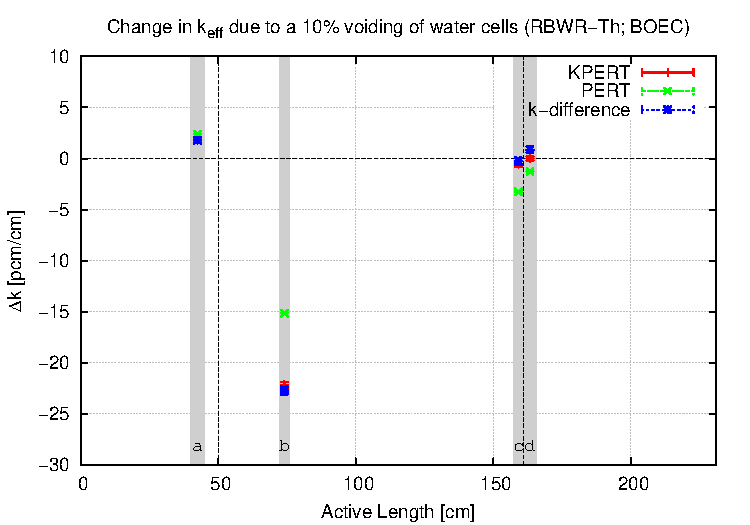
\includegraphics[width=\textwidth, trim=0 0 0 0.275in, clip]{./img/Th-Verify.pdf}
  \caption{Reactivity response from a 10\% local voiding of coolant density, estimated with KPERT, PERT, and k-difference. The KPERT estimate for the perturbation at position $a$ exactly matches k-difference, so the markers overlap. Perturbations at positions $c$ and $d$ are not discussed in this work.}
  \label{fig:verify}
\end{figure}

\clearpage
\begin{figure}[p]
  \centering
  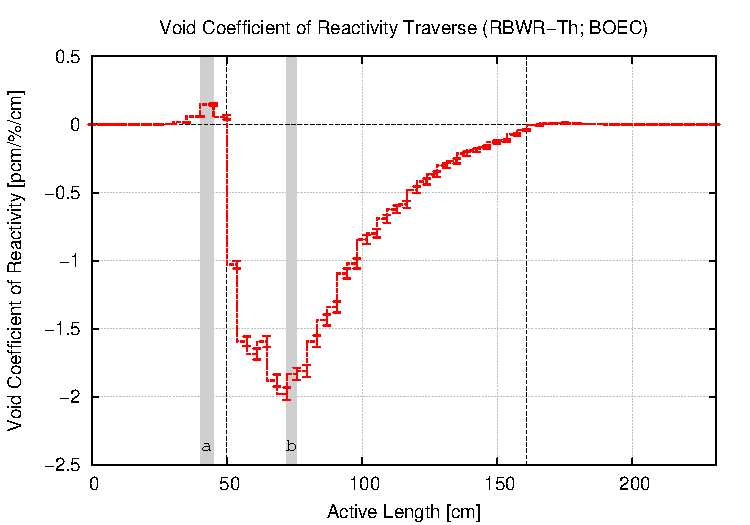
\includegraphics[width=\textwidth, trim=0 0 0 0.275in, clip]{./img/Th-KPERT.pdf}
  \caption{Axial traverse of RBWR-Th local VCRs estimated with KPERT. Perturbations $a$ and $b$ have the most positive and negative reactivity worths.}
  \label{fig:kpert}
\end{figure}

\clearpage
\begin{figure}[p]
  \centering
  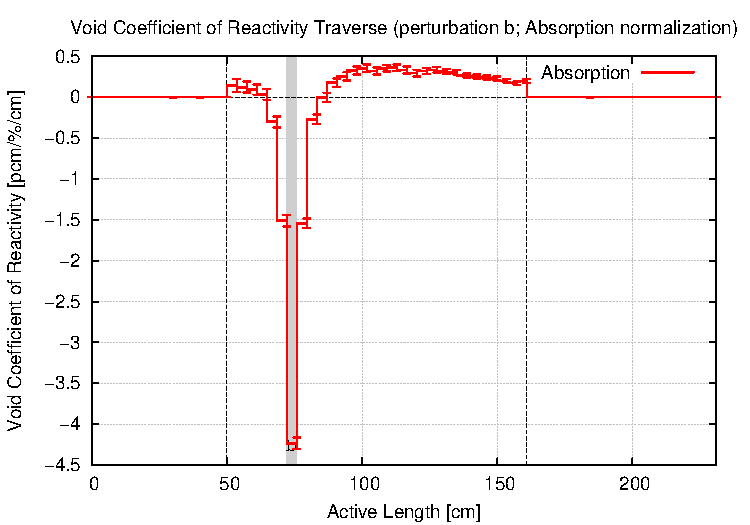
\includegraphics[width=\textwidth, trim=0 0 0 0.275in, clip]{./img/Th-b-TraverseAlphaA.pdf}
  \caption{Absorption-normalized estimate ($\alpha_\A$) for the contribution from axial regions to the VCR due to local void perturbation $b$. Effectively shown are the changes in fission neutron births per neutron absorbed in the entire system.}
  \label{fig:alphaAR}
\end{figure}

\clearpage
\begin{figure}[p]
  \centering
  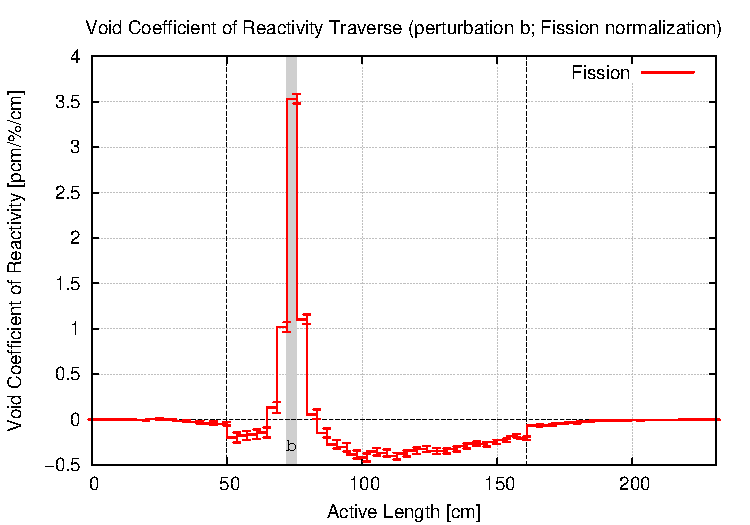
\includegraphics[width=\textwidth, trim=0 0 0 0.275in, clip]{./img/Th-b-TraverseAlphaF.pdf}
  \caption{Fission-normalized estimate ($\alpha_\F$) for the contribution from axial regions to the reactivity response to local void perturbation $b$. Effectively shown are the changes in neutron absorptions per fission neutron born in the entire system.}
  \label{fig:alphaFR}
\end{figure}

\clearpage
\begin{figure}[p]
  \centering
  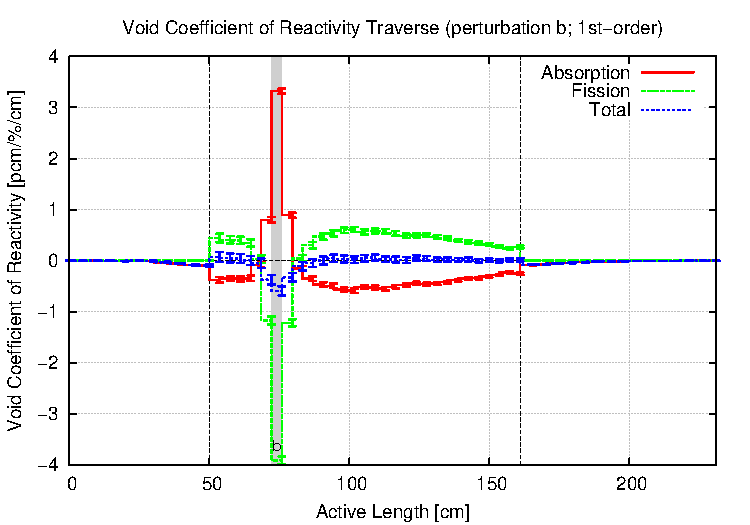
\includegraphics[width=\textwidth, trim=0 0 0 0.275in, clip]{./img/Th-b-TraverseAlpha1.pdf}
  \caption{First-order estimate ($\alpha_1$) of the contribution from axial regions to the reactivity response to local void perturbation $b$. Effectively shown are changes in fission neutron births, neutron absorptions, and their net sum.}
  \label{fig:alpha1R}
\end{figure}

\clearpage
\begin{figure}[p]
  \centering
  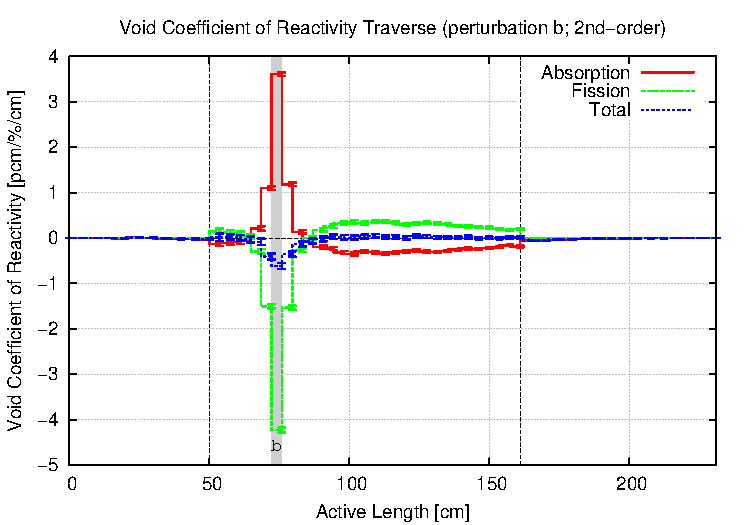
\includegraphics[width=\textwidth, trim=0 0 0 0.275in, clip]{./img/Th-b-TraverseAlpha2.pdf}
  \caption{Second-order estimate ($\alpha_2$) of the contribution from axial regions to the reactivity response to local void perturbation $b$. Effectively shown are changes in fission neutron births, neutron absorptions, and their net sum.}
  \label{fig:alpha2R}
\end{figure}

\clearpage
\begin{figure}[p]
  \centering
  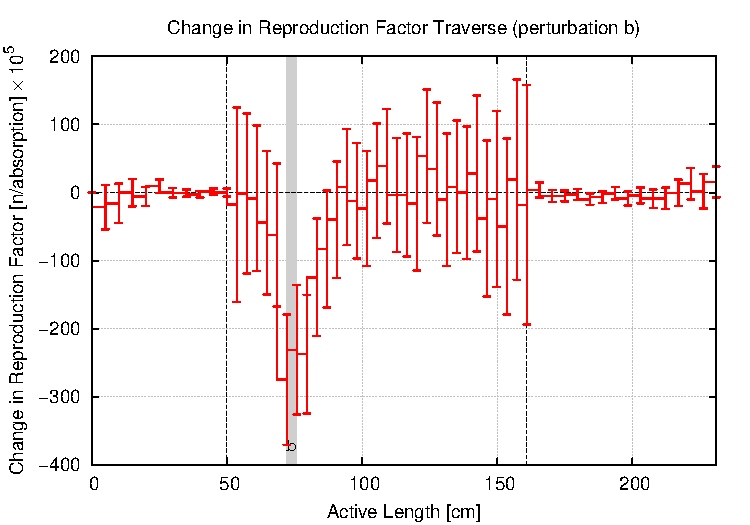
\includegraphics[width=\textwidth, trim=0 0 0 0.275in, clip]{./img/Th-b-TraverseDeltaEta.pdf}
  \caption{Change in the axial reproduction factor ($\eta_r$) due to perturbation $b$. Voiding reduces $\eta_r$ locally but otherwise does not affect $\eta_r$ values.}
  \label{fig:deltaEtaR}
\end{figure}

\clearpage
\begin{figure}[p]
  \centering
  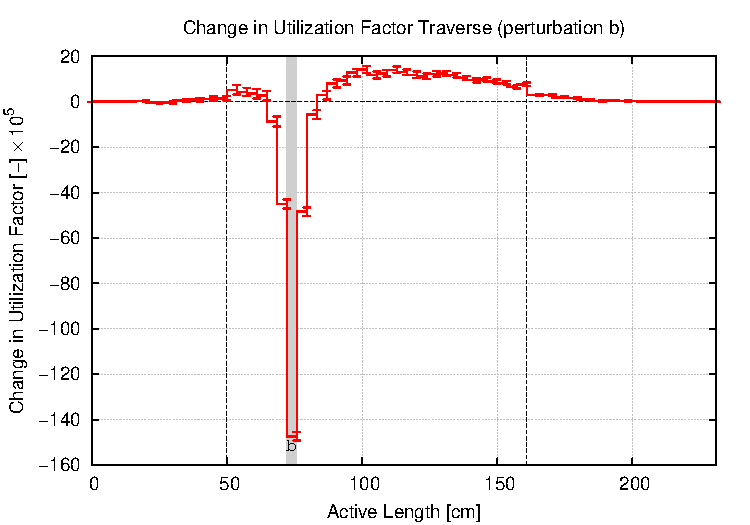
\includegraphics[width=\textwidth, trim=0 0 0 0.275in, clip]{./img/Th-b-TraverseDeltaEff.pdf}
  \caption{Change in the axial utilization factor ($f_r$) due to perturbation $b$. Voiding shifts $f_r$ from the perturbation vicinity to, primarily, upper part of the seed.}
  \label{fig:deltaEffR}
\end{figure}

\clearpage
\begin{figure}[p]
  \centering
  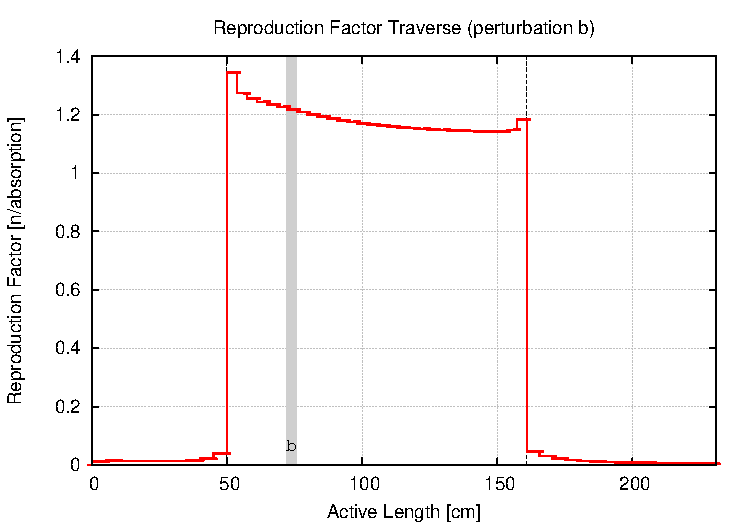
\includegraphics[width=\textwidth, trim=0 0 0 0.275in, clip]{./img/Th-b-TraverseEta.pdf}
  \caption{The RBWR-Th axial reproduction factor ($\eta_r$) is highest near the coolant inlet and decreases with elevation due to coolant boiling.}
  \label{fig:etaR}
\end{figure}

\clearpage
\begin{table}[ht]
    \centering
    \caption{Deviations of estimates for the total reactivity worth of perturbation $b$, between predicted by each of the four perturbation expressions and the k-difference expression. p-values quantify the statistical significance of each deviation.}
    \label{tab:deltaAlpha}
    \begin{tabular}{| c | c | c |} \hline
    \textbf{Expression} & \textbf{Deviation from}     & \textbf{p-value} \\
                        & \textbf{delta-k $[pcm/\%]$} & \textbf{$[\%]$}  \\ \hline
    $\alpha_\A$         & $0.00 \pm 1.1$              & $50$             \\ \hline
    $\alpha_\F$         & $0.00 \pm 1.0$              & $50$             \\ \hline
    $\alpha_1$          & $0.00 \pm 1.4$              & $50$             \\ \hline
    $\alpha_2$          & $0.05 \pm 1.1$              & $52$             \\ \hline
    \end{tabular}
\end{table}

\clearpage
\begin{figure}[p]
  \centering
  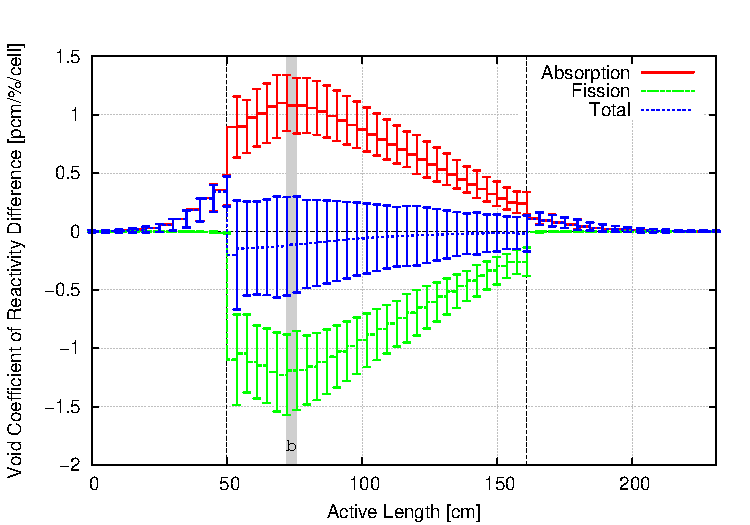
\includegraphics[width=\textwidth, trim=0 0 0 0.275in, clip]{./img/Th-b-Traverse12Cmp.pdf}
  \caption{Difference between the second-order ($\alpha_2$) and first-order ($\alpha_1$) (calculated as $\alpha_2-\alpha_1$) estimates of the contribution from axial regions to the reactivity response to local void perturbation $b$. Due to the small difference between the two estimates, Monte Carlo counting uncertainties are relatively large.}
  \label{fig:deltaAlphaR}
\end{figure}

\clearpage
\begin{figure}[p]
  \centering
  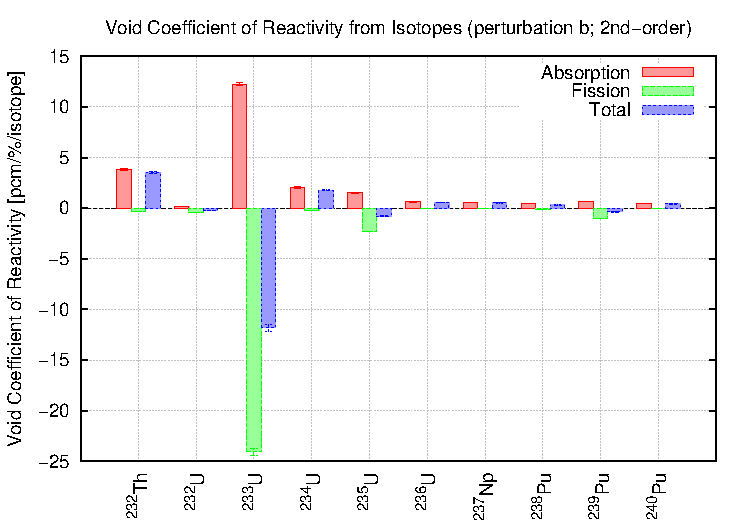
\includegraphics[width=\textwidth, trim=0 0 0 0.275in, clip]{./img/Th-b-IsotopeAlpha2.pdf}
  \caption{Localized isotopic contribution to perturbation $b$'s local VCR. The net reactivity worths contributed by fissile isotopes are negative while those from non-fissile isotopes are positive.}
  \label{fig:alpha2I}
\end{figure}

\clearpage
\begin{figure}[p]
  \centering
  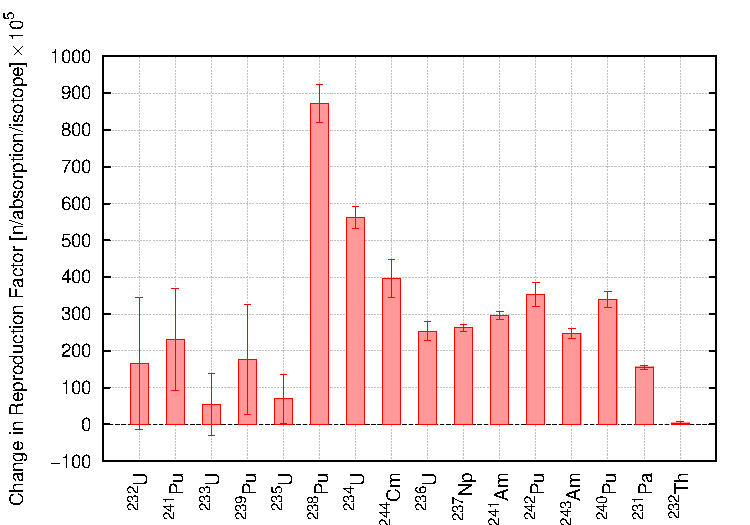
\includegraphics[width=\textwidth, trim=0 0 0 0, clip]{./img/Th-b-IsotopeDeltaEta.pdf}
  \caption{Localized change in isotopic reproduction factors $\eta_i$ due to perturbation $b$. All values are positive.}
  \label{fig:deltaEtaI}
\end{figure}

\clearpage
\begin{figure}[p]
  \centering
  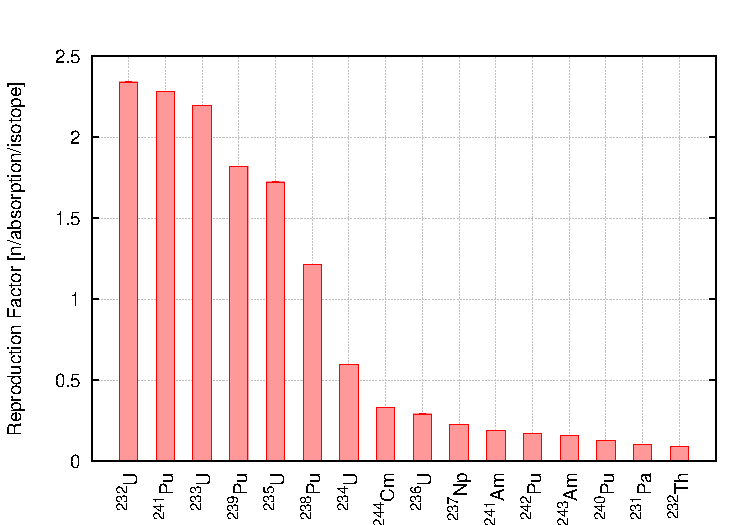
\includegraphics[width=\textwidth, trim=0 0 0 0.275in, clip]{./img/Th-b-IsotopeEta.pdf}
  \caption{Isotopic reproduction factors $\eta_i$, in proximity to perturbation $b$.}
  \label{fig:etaI}
\end{figure}

\clearpage
\begin{figure}[p]
  \centering
  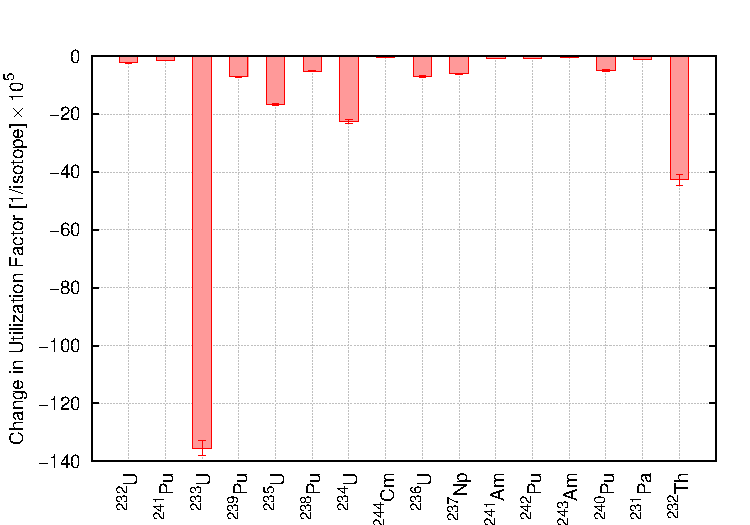
\includegraphics[width=\textwidth, trim=0 0 0 0.275in, clip]{./img/Th-b-IsotopeDeltaEff.pdf}
  \caption{Change in isotopic utilization factors $f_i$, in proximity to perturbation $b$.}
  \label{fig:deltaEffI}
\end{figure}

\clearpage
\begin{figure}[p]
  \centering
  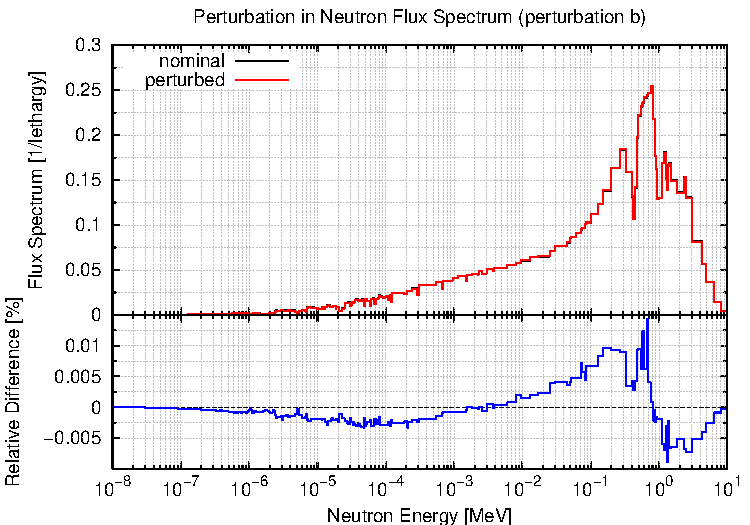
\includegraphics[width=\textwidth, trim=0 0 0 0.2in, clip]{./img/Th-b-SpectraFlux.pdf}
  \caption{Localized change in flux spectrum due to perturbation $b$, normalized to an integral of unity.}
  \label{fig:deltaFlx}
\end{figure}

\clearpage
\begin{figure}[p]
  \centering
  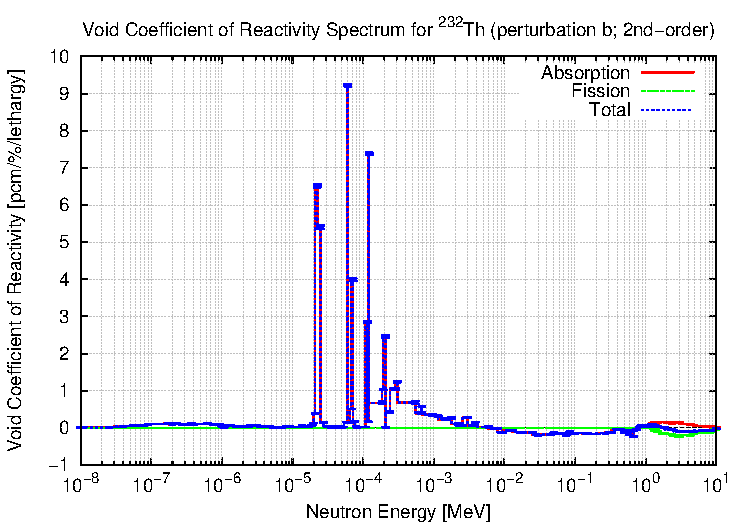
\includegraphics[width=\textwidth, trim=0 0 0 0.275in, clip]{./img/Th-b-SpectraAlpha2-Th-232.pdf}
  \caption{Localized \iso{Th}{232} energy-dependent contribution to perturbation $b$'s VCR. An overall positive reactivity response results from reduced resonance-energy absorptions.}
  \label{fig:alphaETh}
\end{figure}

\clearpage
\begin{figure}[p]
  \centering
  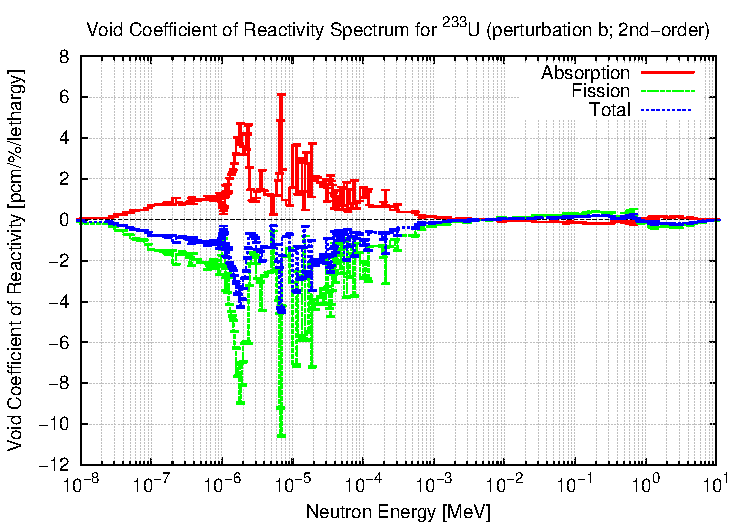
\includegraphics[width=\textwidth, trim=0 0 0 0.275in, clip]{./img/Th-b-SpectraAlpha2-U-233.pdf}
  \caption{Localized \iso{U}{233} energy-dependent contribution to perturbation $b$'s VCR. An overall negative reactivity response is due to reduced thermal and epithermal fissions.}
  \label{fig:alphaEU}
\end{figure}

\clearpage
\begin{figure}[p]
  \centering
  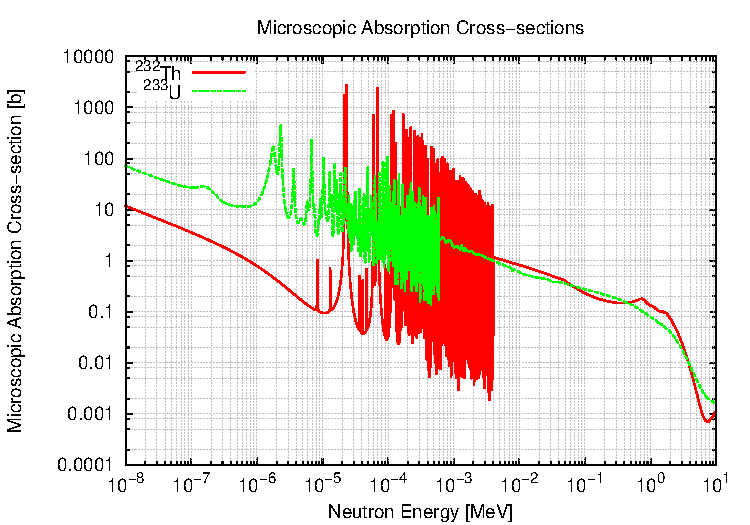
\includegraphics[width=\textwidth, trim=0 0 0 0.275in, clip]{./img/XsAbsorption.pdf}
  \caption{Energy dependent absorption cross section of \iso{Th}{232} and \iso{U}{233}.}
  \label{fig:xs}
\end{figure}

\clearpage
\begin{figure}[p]
  \centering
  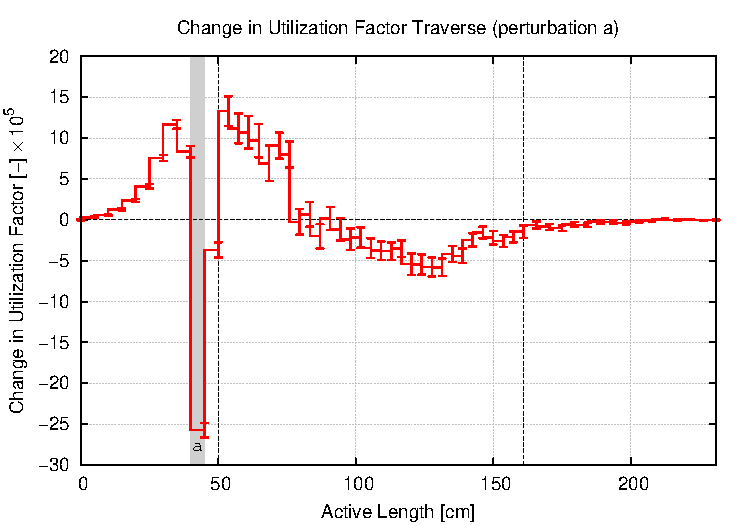
\includegraphics[width=\textwidth, trim=0 0 0 0.275in, clip]{./img/Th-a-TraverseDeltaEff.pdf}
  \caption{Change in the local utilization factor $f_r$ due to perturbation $a$. Voiding shifts $f_r$ from the top to the bottom of the core.}
  \label{fig:deltaEffRb}
\end{figure}

\clearpage
\begin{figure}[p]
  \centering
  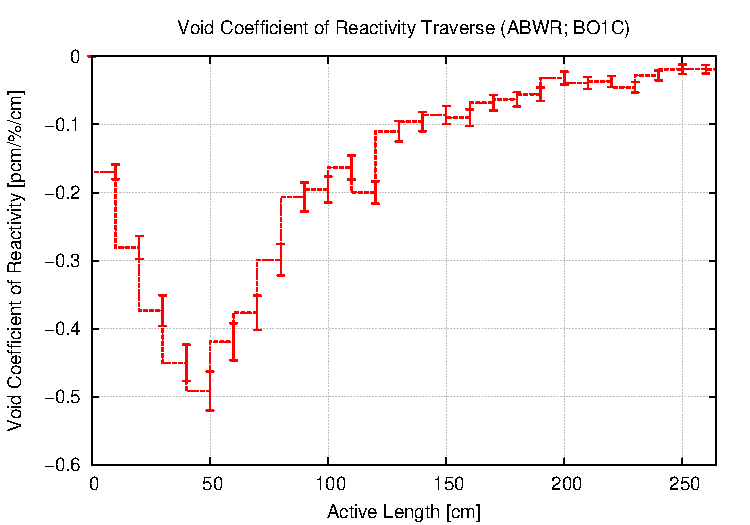
\includegraphics[width=\textwidth, trim=0 0 0 0.275in, clip]{./img/ABWR-KPERT.pdf}
  \caption{Axial traverse of ABWR local VCRs estimated with KPERT. The overall shape is similar to that of the RBWR-Th seed region, shown in Fig. \ref{fig:kpert}.}
  \label{fig:kpertAbwr}
\end{figure}

\clearpage
\begin{figure}[p]
  \centering
  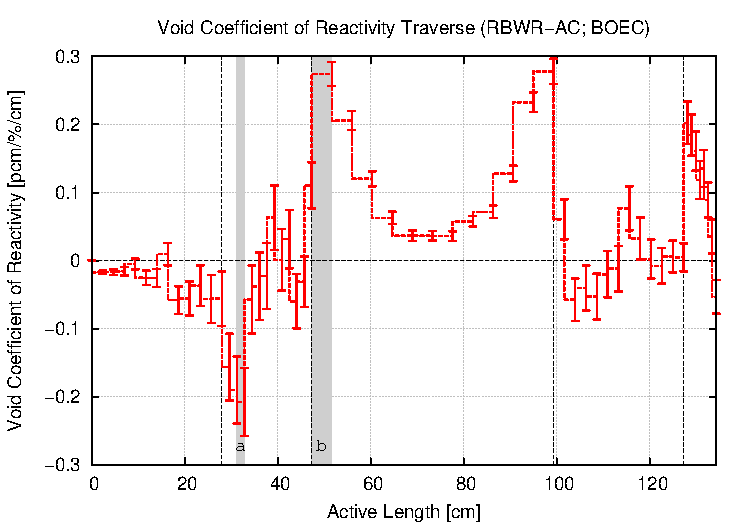
\includegraphics[width=\textwidth, trim=0 0 0 0.275in, clip]{./img/AC-KPERT.pdf}
  \caption{Axial traverse of RBWR-AC local VCRs estimated with KPERT. Perturbations $a$ and $b$ result in the most negative and positive reactivity worth. The seed regions -- from $28$ to $47.3cm$ and from $99.3$ to $127.3cm$, are sandwiched between the three axial blanket regions.}
  \label{fig:kpertAc}
\end{figure}

\clearpage
\begin{figure}[p]
  \centering
  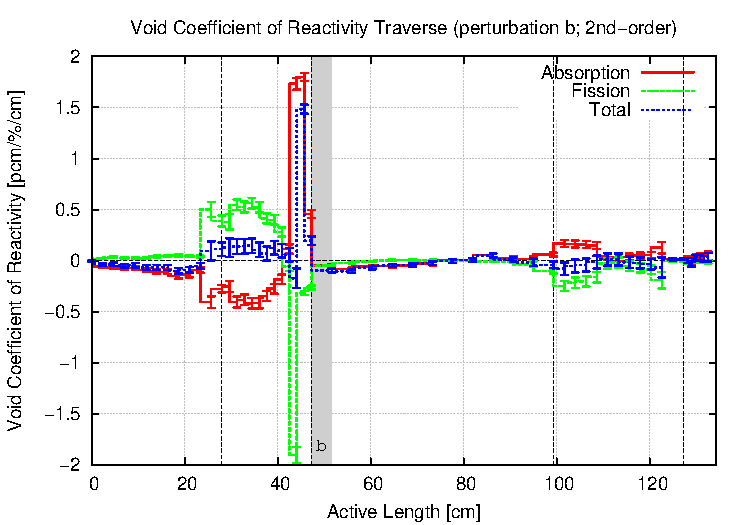
\includegraphics[width=\textwidth, trim=0 0 0 0.275in, clip]{./img/AC-TraverseAlpha2.pdf}
  \caption{Total contribution from axial fuel regions to the reactivity response to local void perturbation $b$.}
  \label{fig:alphaAc}
\end{figure}

\clearpage
\begin{figure}[p]
  \centering
  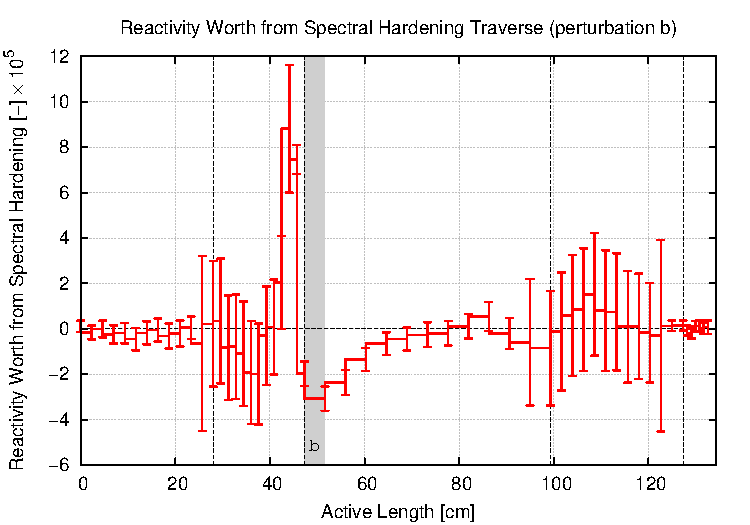
\includegraphics[width=\textwidth, trim=0 0 0 0.275in, clip]{./img/AC-TraverseDeltaEtaEff.pdf}
  \caption{Spectral hardening contribution ($\sum_r{\Delta\eta_r f_r}$) from axial fuel regions to the reactivity response to local void perturbation $b$.}
  \label{fig:spectralAc}
\end{figure}

\clearpage
\begin{figure}[p]
  \centering
  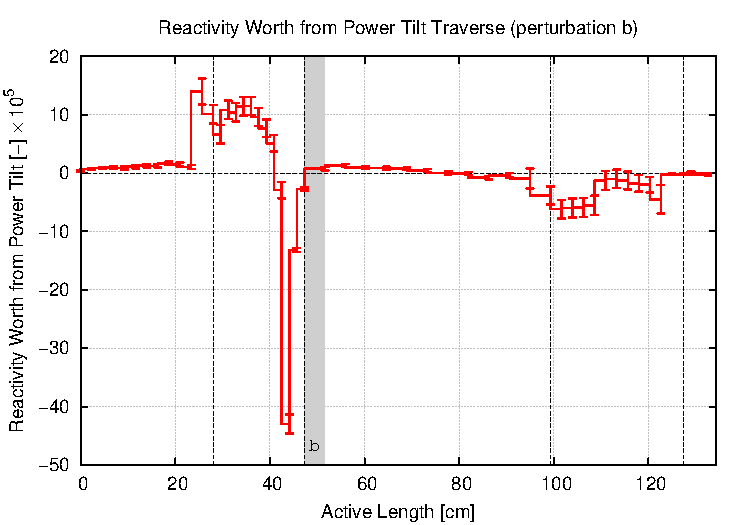
\includegraphics[width=\textwidth, trim=0 0 0 0.275in, clip]{./img/AC-TraverseEtaDeltaEff.pdf}
  \caption{Flux tilt contribution ($\sum_r{\eta_r \Delta f_r}$) from axial fuel regions to the reactivity response to local void perturbation $b$.}
  \label{fig:tiltAc}
\end{figure}

\end{document}
